\chapter{Introduction} \label{chap:introduction}

%The aim of this project is to investigate the possibilities of a novel concept of airfoil twist morphing.

%Describe a little bit what is morphing...
The interest in morphing of the aerodynamic surfaces has accompany aerospace history since the beginning. Since the first heavier-than-air flight in 1903, when the Wright Brothers designed and build a powered heavier-than-air aircraft that achieved the  first controlled and sustained flight. Their concept of aircraft did not provide importance to built-in stability but absolute control of the aircraft by the pilot. For this reason, they deliberatively designed their first aircraft with anhedral wing that make it dynamically unstable to perturbations in sideslip but more maneuverable in the lateral direction. In order to achieve roll control, they decided to incorporate a mechanism that would allow the wings to twist by pulling from cables, as it can be seen in Figure \ref{fig:Wright}. This was the first ever use of morphing of an aerodynamic surface for aircraft control. Since them, the necessity of enhanced performance and higher airspeed brought the requirement of stiffer wing structures to avoid aeroelastic instabilities.

\begin{figure}[!htpb]
  \centering
  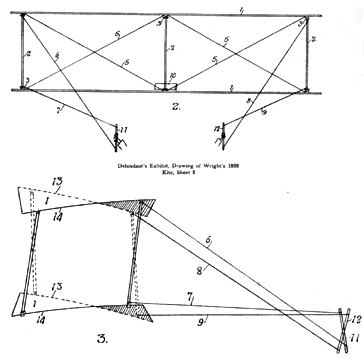
\includegraphics[width=0.6 \textwidth]{state-of-the-art/WrightBrothers1899Kite}
  \caption[Wright Brothers 1899 kite]{Wright Brothers 1899 kite: front and side views, with control sticks. Wing-warping is shown in lower view. \cite{Wright}}\label{fig:Wright}
\end{figure}

%Why to used them?
On conventional aircraft, the need to modify the airflow around the airfoil at different flight conditions is achieved through discrete hinged mechanics such as flaps and ailerons. These mechanism performs well in a limited range around the design point while the outside this range, they have a negative influence in the aerodynamics. The necessary discontinuities that these elements produce on the surface, advance the boundary layer transition point from laminar to turbulent regime. Being able to modify the airflow without discontinuities on the surface would come along with notable reductions in parasite drag and therefore in fuel consumption.

%Gust
Under certain flight conditions, the aircraft may experience critical loads that mark the design point for the airframe due to its structural integrity threat. One of this condition is gust encountering. In this situation the aircraft is flying in turbulent air and a component of the velocity of air normal to the flight path, changes the effective angle of incidence of the aerodynamic surfaces increasing its aerodynamic load. In Figure \ref{fig:gust}, the case of an aircraft encountering a vertical gust is shown. Several mechanisms which usually add structural mass have been develop to withstand this rare scenarios. The requirements of such of solutions require of a rapid modification of the lift distribution that mitigates the impact of such events. In modern transonic aircraft, after a gust encountering, the ailerons of both wings are deflected in such a way that they reduce the local airfoil chamber, reducing as well the lift generated at the wing tip.

\begin{figure}[!htpb]
  \centering
  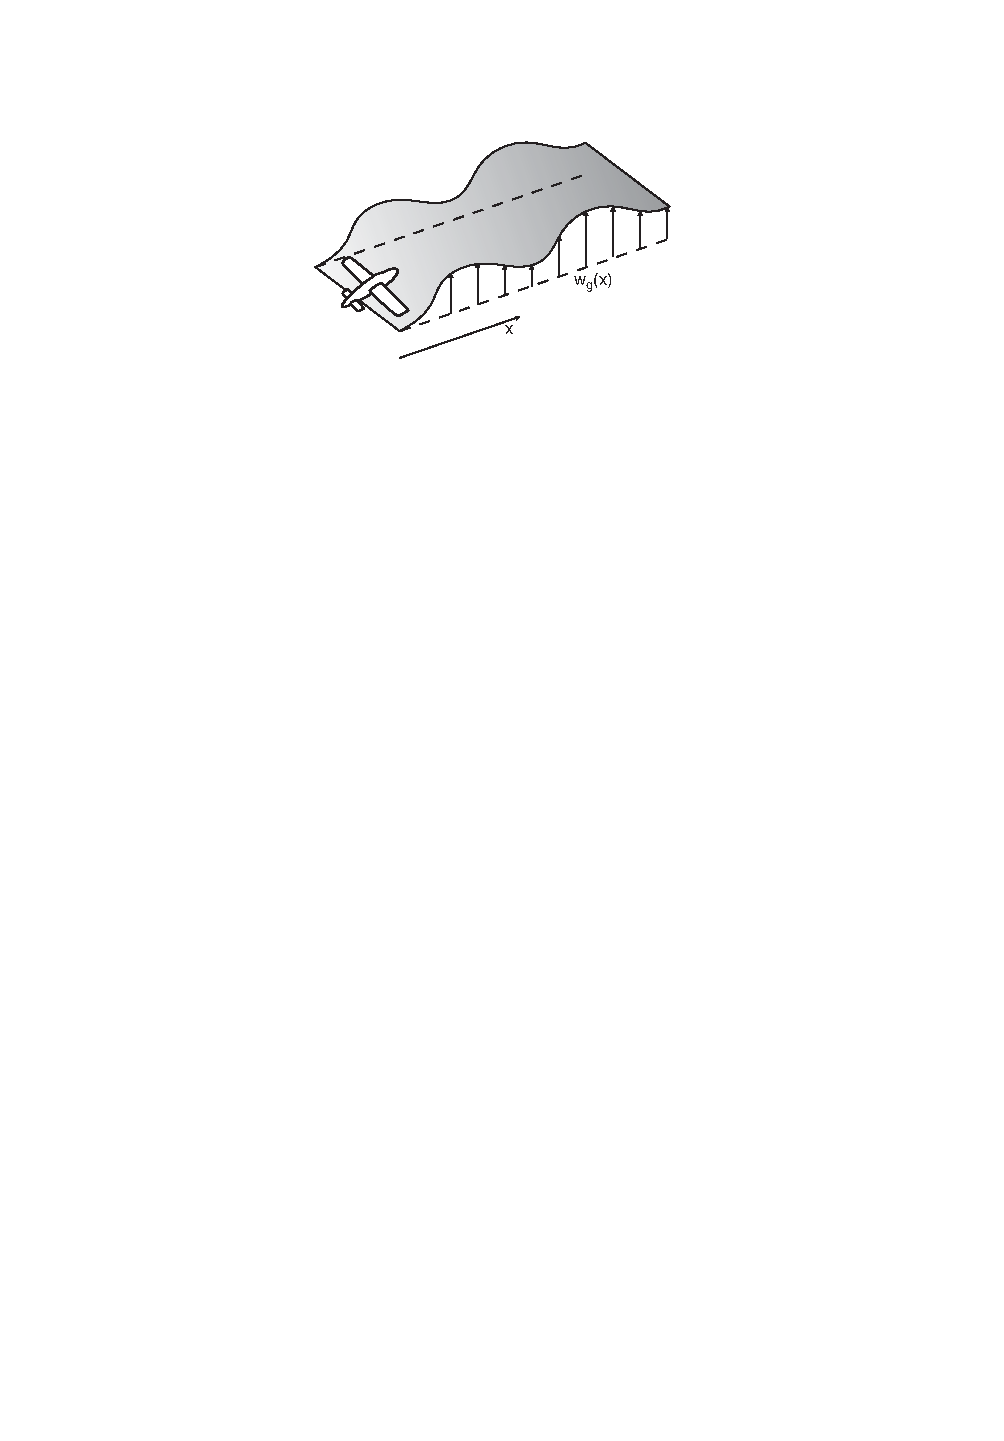
\includegraphics[width=0.7 \textwidth]{state-of-the-art/gust}
  \caption[Aircraft encountering a vertical gust]{Aircraft encountering a vertical gust. \cite{JECooper2007}}\label{fig:gust}
\end{figure}

Furthermore, the use of wing morphing in a attempt to modify wing geometrical parameters of relevance such as the twist and provide gust load alleviation, has been always something of interest for researches. These type of solutions show compliance with the response requirement exposed in  previous paragraph, in addition of having advantages such as the weight reduction and/or the no alteration of the aerodynamic surfaces continuity with hinges, providing reduced operation costs and aerodynamic performance enhancement, respectively. 

The present work is a proposal of a novel wing morphing technology that enables the rapid alteration of the wing twist. This alteration would reduce the angle of attack and therefore would limit the aerodynamic load on the wings. The presented concept consists on the alteration of the torsional stiffness of the wing-box of the wing by the inclusion of a variable-stiffness spar. The modification of the effective shear modulus in this element provokes the wing-box's center shifting. This event is fully passively activated and its based on the appearance of elastic controlled instabilities in the structure of the variable-stiffness spar.

The objectives for the work presented in this thesis include on first place the evaluation of the buckling mechanism as a valid trigger for the variable-stiffness spar adaptation and consequent variation of the wing-box twist. Secondly, the elastic instability or buckling that undergoes in the spar is aimed to be characterized by qualitative means. Finally, the possibility of tailoring the deformation response by varying the structure parameters is intended to be evaluated. 

This thesis is organized as follows: succeeding this introduction, the state-of-the-art of the technologies related to the one proposed in this work are presented. Then, the wing-box model that has been developed to investigated the suggested concept is explained in the third chapter, following a characterization of its mechanical properties in the subsequent chapter. The fifth chapter shows the results obtained from the simulations performed on the computational model of the wing-box. The conclusion and outlook complete this thesis.